\label{sec::4_he}
Heicub is a descendant of the iCub, which was specially designed for optimal control in locomotion at the Istituto Italiano di Tecnologia in Genova. It is used within this thesis to test the implemented algorithms, for which it provides all the required actuators and sensors. As shown in figure \ref{fig::4_hei} (c), Heicub has a total of 21 degrees of freedom, of which six correspond to the floating base, and 15 to the rotational joints. 
\begin{figure}[h!]
	\centering
	\subcaptionbox{Heicub.}%
	[.3\linewidth]{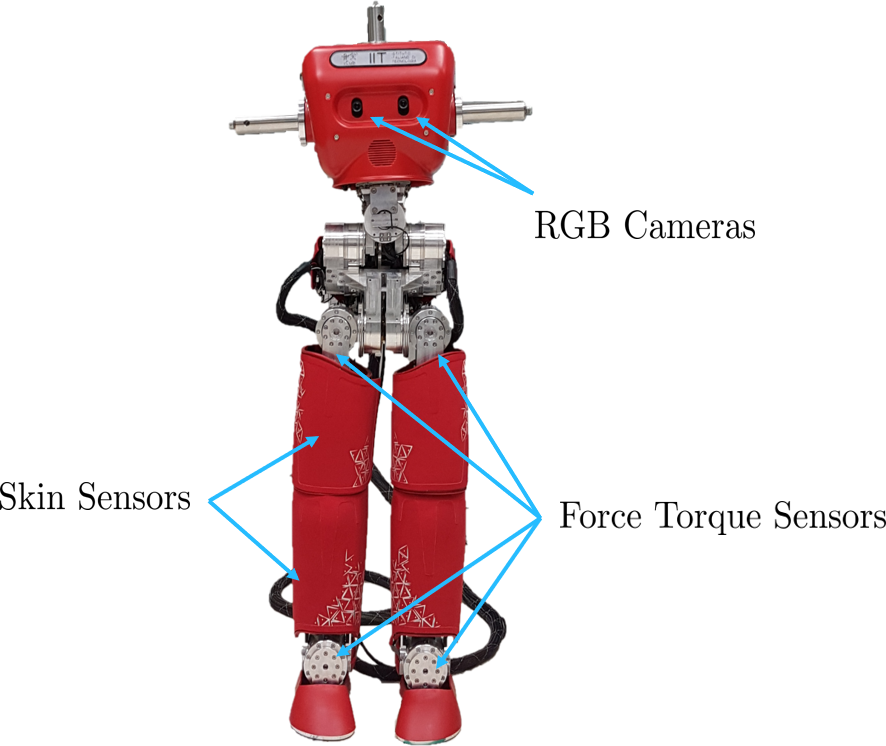
\includegraphics[scale=.35]{chapters/05_heicub_our_humanoid_robot/img/heicub.png}}
	\subcaptionbox{Gazebo model.}%
	[.3\linewidth]{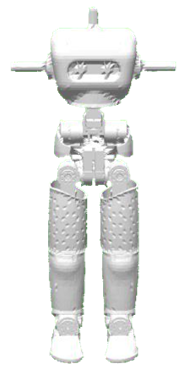
\includegraphics[scale=.35]{chapters/05_heicub_our_humanoid_robot/img/gazebo_heicub.png}}
	\subcaptionbox{Kinematic chain.}%
	[.3\linewidth]{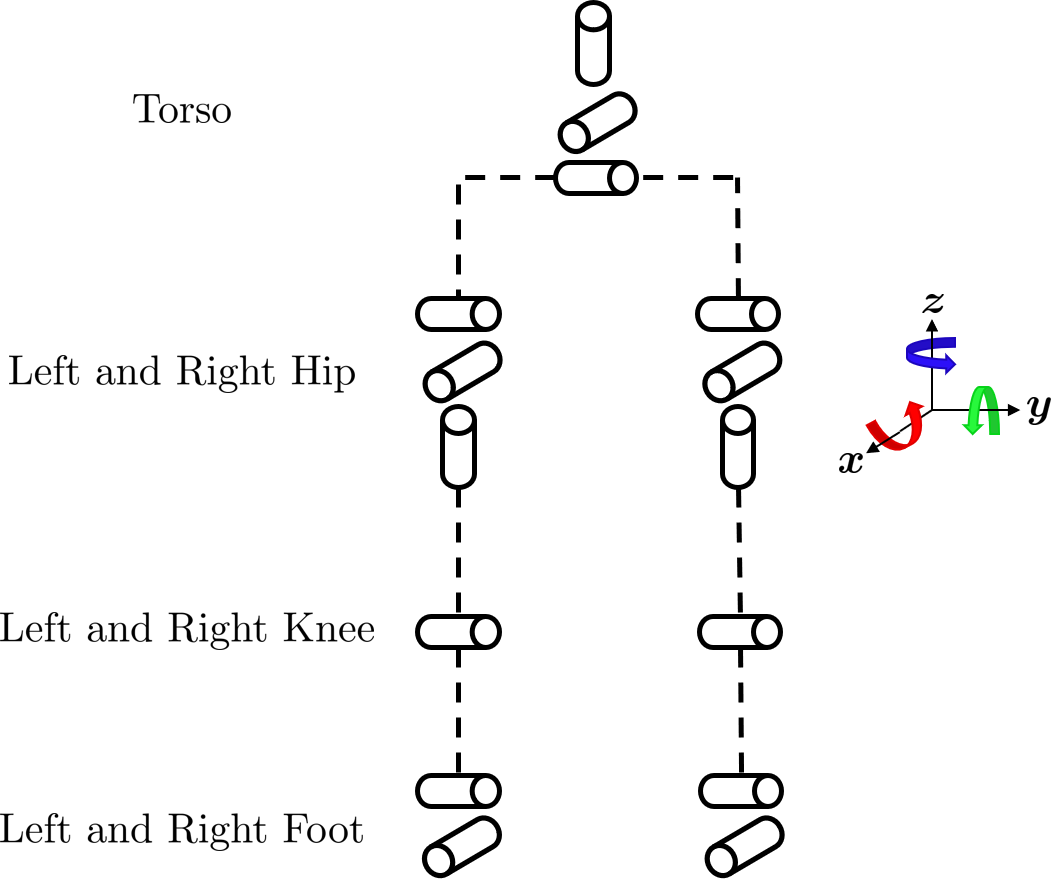
\includegraphics[scale=.35]{chapters/05_heicub_our_humanoid_robot/img/kinematic_tree.png}}
	\caption{Heicub, the robot, which we used for the evaluation of the implemented software. There exists the real robot (a), as well as a simulated version of it, which offer equivalent functionality (b). Heicub's degrees of freedom, which can be actuated, are shown in (c). All the joints are rotational joints.}
	\label{fig::4_hei}
\end{figure}
Its two RGB cameras have a resolution of $240\times320$ pixels at a framerate of $60\,\text{fps}$, and are located within the chest, as shown in figure \ref{fig::4_hei} (a). The force-torque sensors, with which we compute the zero moment point, are located within the ankles and the hip. According to equations \ref{eq::21_x_pos_zmp_simp} and \ref{eq::21_y_pos_zmp_simp}, we only require the force-torque sensors from the ankles, where $d=0.03\,\text{m}$. Heicub also supports skin sensors, and an inertial measurement unit, but both are not used within this thesis. The use of the robot, and all its sensors, is well described within the appendix, starting from section \ref{sec::B_su}. It is possible to communicate with Heicub via YARP \cite{metta2006yarp}, which is short for Yet Another Robot Platform, and its installation is explained in section \ref{sec::a52_yarp}. Furthermore, Heicub has a Gazebo \cite{koenig2004design} simulation model, which is shown in figure \ref{fig::4_hei} (b), and for which the installation instructions can be found in section \ref{sec::A4_sm}. It provides the exact same functionality as its real equivalent does. This is achieved via Gazebo plugins, which communicate to the YARP network, just as Heicub does. The plugins can be installed by following the instructions in section \ref{sec::a52_plugins}. The Gazebo model offers a perfect environment for software development, as we can make sure that implemented algorithms work properly, prior to their usage on the real robot, which could take harm from wrongly designed software.